\documentclass[oneside,a4paper,14pt]{extarticle}
\usepackage[a4paper,letterpaper,top=20mm,bottom=20mm,left=20mm,right=10mm]{geometry}
\usepackage[russian]{babel}
\usepackage{indentfirst}
\usepackage{graphicx}
\usepackage{caption}
\usepackage{titlesec}
\usepackage{minted, fancyvrb}
\usepackage{hyperref}
\usepackage{enumitem}

% Форматирование листингов с кодом
\setminted{style = rainbow_dash, fontsize = \small} % https://pygments.org/styles/

% Форматирование заголовков
\titleformat{\section}{\normalsize\bfseries}{\thesection}{1em}{}
\titleformat{\subsection}{\normalsize\bfseries}{\thesubsection}{1em}{}
\titleformat{\subsubsection}{\normalsize\bfseries}{\thesubsubsection}{1em}{}

% Интерлиньяж и абзац
\renewcommand\baselinestretch{1.33}

\setlength{\parindent}{1.25cm}  % длина красной строки

% Для всех списков
\setlist[enumerate]{
  left=0.5\parindent,       % отступ слева
  label=\arabic*.,       % цифры
  itemsep=0pt,           % расстояние между пунктами
  topsep=5pt,            % отступ сверху
  partopsep=0pt,         % дополнительный отступ сверху, если абзац до списка
  parsep=0pt             % отступ между абзацами внутри пункта
}

\setlist[itemize]{
  left=0.5\parindent,       % отступ слева
  itemsep=0pt,           % расстояние между пунктами
  topsep=5pt,            % отступ сверху
  partopsep=0pt,
  parsep=0pt
}

% Гиперссылки
\hypersetup{
  colorlinks=true,
  linkcolor=black,
  urlcolor=blue,
  pdfborder={0 0 0},
  pdftitle={PyQt6 приложение для управления устройствами умного дома},
  pdfauthor={Черкасов А.А.}
}

\begin{document}

\newpage
\thispagestyle{empty}
\begin{center}
  МИНИСТЕРСТВО НАУКИ И ВЫСШЕГО ОБРАЗОВАНИЯ РОССИЙСКОЙ ФЕДЕРАЦИИ ФЕДЕРАЛЬНОЕ ГОСУДАРСТВЕННОЕ БЮДЖЕТНОЕ ОБРАЗОВАТЕЛЬНОЕ УЧРЕЖДЕНИЕ ВЫСШЕГО ОБРАЗОВАНИЯ\\
  «ВЯТСКИЙ ГОСУДАРСТВЕННЫЙ УНИВЕРСИТЕТ»\\
  Институт математики и информационных систем\\
  Факультет автоматики и вычислительной техники\\
  Кафедра электронных вычислительных машин
\end{center}
\vspace{10mm}

\hfill
\begin{tabular}{l}
  \footnotesize Дата сдачи на проверку:                                          \\
  \footnotesize <<\rule[-1mm]{5mm}{0.10mm}\/>>\rule[-1mm]{20mm}{0.10mm}\ 2025 г. \\
  \footnotesize Проверено:                                                       \\
  \footnotesize <<\rule[-1mm]{5mm}{0.10mm}\/>>\rule[-1mm]{20mm}{0.10mm}\ 2025 г. \\
\end{tabular}
\vfill

\begin{center}
  Отчёт по лабораторной работе №1\\
  по дисциплине\\
  <<Теория Автоматов>>\\
\end{center}
\vspace{25mm}
\noindent
\begin{tabular}{ll}
  Разработал студент гр. ИВТб-2301-05-00 & \hspace{18mm}\rule[-1mm]{30mm}{0.10mm}\,/Черкасов А. А./ \\
                                         & \hspace{25.5mm}\footnotesize(подпись)                    \\
  Старший Преподователь                  & \hspace{18mm}\rule[-1mm]{30mm}{0.10mm}\,/Мельцов В. Ю./  \\
                                         & \hspace{25.5mm}\footnotesize(подпись)                    \\
\end{tabular}

\noindent
\begin{tabular}{lp{58mm}r}
  Работа защищена &  & \hspace{13mm}<<\rule[-1mm]{5mm}{0.10mm}\/>>\rule[-1mm]{30mm}{0.10mm}\ 2025 г.
\end{tabular}
\vfill

\begin{center}
  Киров\\
  2025
\end{center}

\newpage\thispagestyle{plain}

\section*{Цель лабораторной работы}
Разработка автомата, подающего случайную последовательность входных сигналов.

\section*{Задание}
Разработать автомат, подающий случайную последовательность входных сигналов. Автомат моделирует процесс управления пирамидами с кольцами, где каждая пирамида может находиться в одном из трех состояний:

\begin{enumerate}
  \item \textbf{Начальное состояние (O)}: массив пар (индекс пирамиды, количество колец), задающий начальную конфигурацию.
  \item \textbf{Состояние обработки (P)}: массив пирамид, находящихся в процессе обработки. Изначально копирует состояние O.
  \item \textbf{Завершенное состояние (F)}: массив пирамид, достигших максимального количества колец (12).
\end{enumerate}

\noindent В каждом шаге симуляции автомат выполняет следующие действия:
\begin{itemize}
  \item[$-$] Случайным образом выбирает пирамиду из состояния P и добавляет ей одно кольцо.
  \item[$-$] Если количество колец достигает 12, пирамида перемещается в состояние F.
  \item[$-$] С заданной вероятностью (параметр emergencyChance) вызывает аварийную ситуацию: выбирает случайную пирамиду из P с количеством колец не менее 3 и уменьшает ее кольца на 3.
\end{itemize}

\noindent Создать приложение с графическим интерфейсом на Qt6, позволяющее:
\begin{enumerate}
  \item Настраивать начальное состояние пирамид (количество колец).
  \item Выбирать цвета для визуализации пирамид.
  \item Управлять скоростью симуляции и вероятностью аварий.
  \item Визуализировать текущее состояние пирамид с анимацией.
  \item Сохранять и загружать конфигурации симуляции.
\end{enumerate}

\section*{Реализация приложения}

\begin{figure}[H]
  \centering
  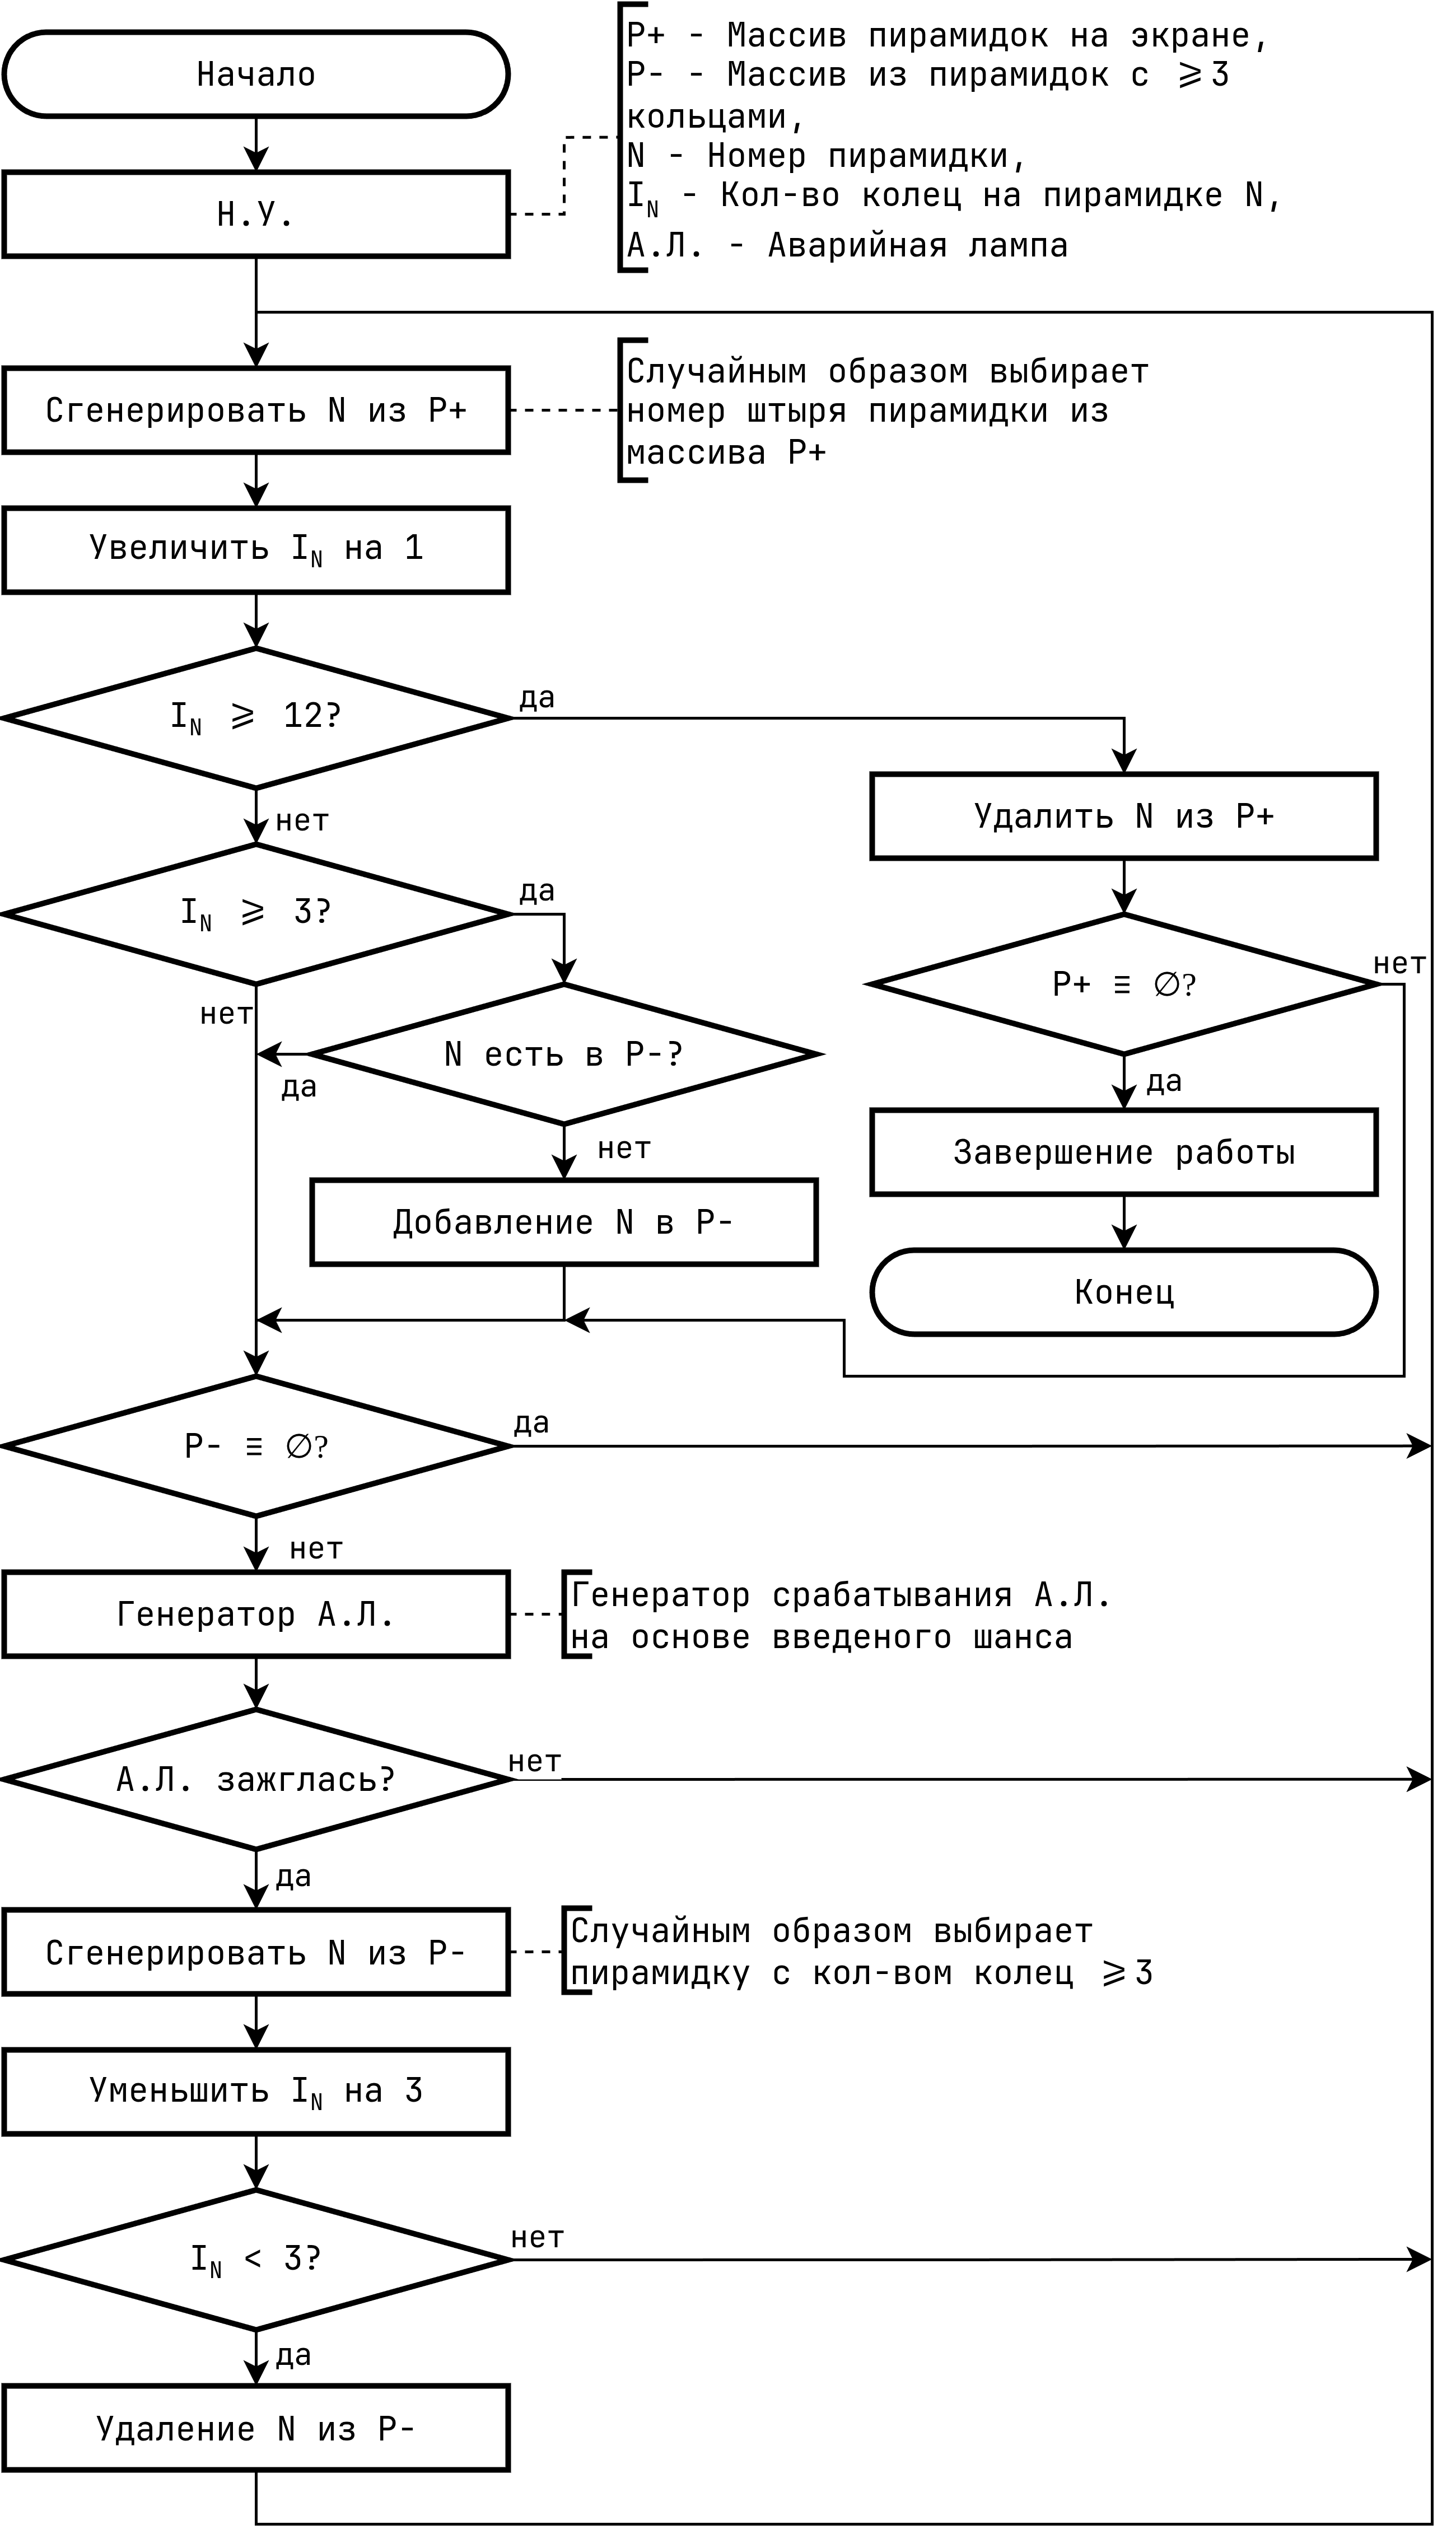
\includegraphics[height=0.9\textheight]{pics/flowchart.png}
  \caption*{Рисунок 1 - Схема алгоритма автомата}
\end{figure}

Архитектура приложения построена на фреймворке Qt6 и включает следующие основные классы:
\begin{itemize}
  \item[$-$] \texttt{Simulation} $-$ класс, реализующий логику автомата с состояниями O, P, F
  \item[$-$] \texttt{MainWindow} $-$ главное окно приложения с пользовательским интерфейсом
  \item[$-$] \texttt{PyramidWidget} $-$ виджет для визуализации пирамид с кольцами и анимацией
  \item[$-$] \texttt{InitialFillDialog} $-$ диалог настройки начального количества колец
  \item[$-$] \texttt{ColorDialog} $-$ диалог выбора цветов пирамид
\end{itemize}

\subsection*{Интерфейс программы}

Главное окно приложения состоит из следующих элементов управления:

\begin{itemize}
  \item[$-$] \textbf{Строка меню} (вверху): содержит меню «Файл» (Открыть, Сохранить, Выход), «Настройки» (Начальное заполнение, Выбор цвета) и «Справка» (О программе, Об авторе).
  \item[$-$] \textbf{Область визуализации пирамид} (центр): 10 виджетов пирамид, расположенных в 2 ряда по 5 штук. Каждая пирамида отображается своим цветом с кольцами.
  \item[$-$] \textbf{Панель управления} (внизу): содержит элементы управления симуляцией.
  \item[$-$] \textbf{Строка состояния} (внизу): показывает количество пирамид в состояниях P и F.
\end{itemize}

Панель управления включает:
\begin{itemize}
  \item[$-$] \textbf{Ползунок «Скорость (тиков/сек)»} (0-100): регулирует скорость симуляции. Значение 0 останавливает симуляцию.
  \item[$-$] \textbf{Поле ввода скорости}: текстовое поле для точного ввода значения скорости с валидацией (только цифры 0-100).
  \item[$-$] \textbf{Ползунок «Шанс аварии (\%)»} (0-100): задает вероятность аварийной ситуации в каждом тике.
  \item[$-$] \textbf{Поле ввода шанса аварии}: текстовое поле для ввода процента аварий с валидацией.
  \item[$-$] \textbf{Кнопка «Старт/Стоп»}: запускает или останавливает симуляцию. При запуске текст меняется на «Стоп».
  \item[$-$] \textbf{Кнопка «Пауза/Продолжить»}: приостанавливает или возобновляет симуляцию. При паузе текст меняется на «Продолжить».
  \item[$-$] \textbf{Кнопка «Выход»}: закрывает приложение.
\end{itemize}

\begin{figure}[H]
  \centering
  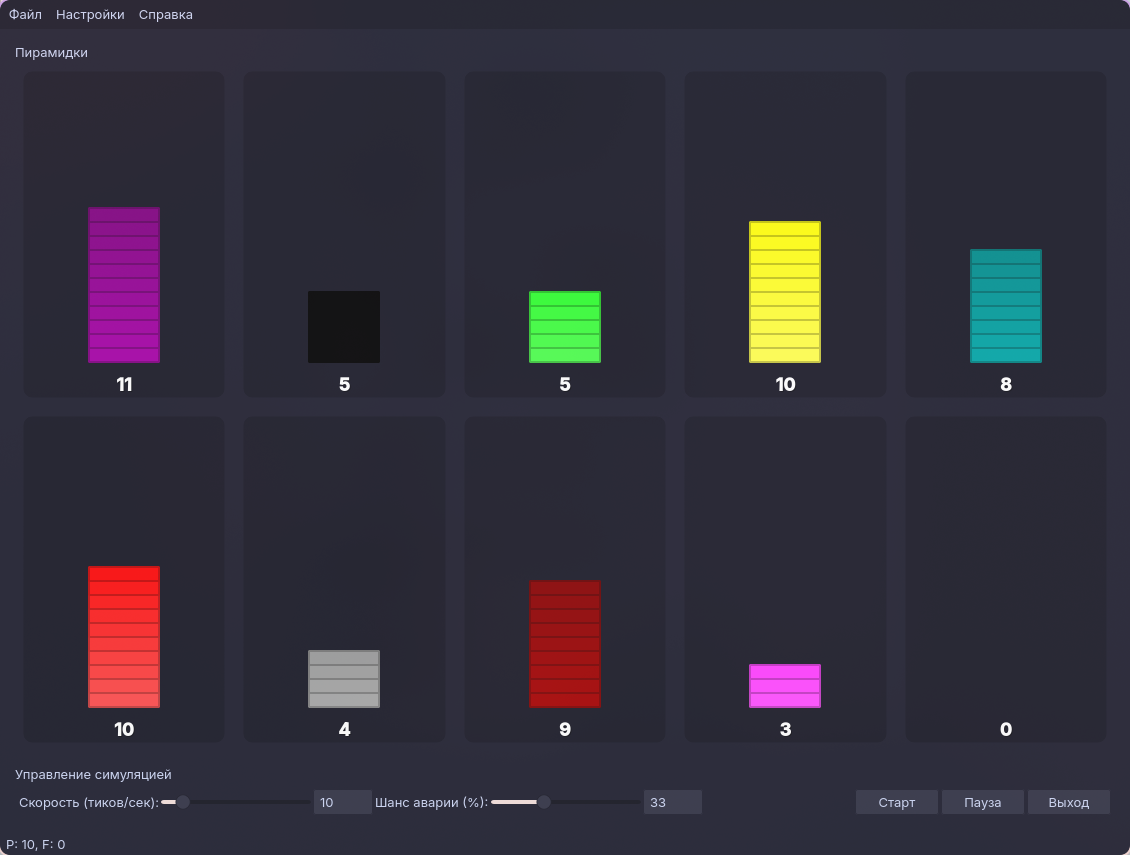
\includegraphics[width=0.95\textwidth]{pics/main_window.png}
  \caption*{Рисунок 2 - Главное окно приложения с визуализацией пирамид}
\end{figure}

Диалог настройки начального количества колец открывается через меню «Настройки → Начальное заполнение». Содержит:

\begin{itemize}
  \item[$-$] \textbf{10 полей ввода} (QSpinBox) для каждой пирамиды с диапазоном 0-11 колец.
  \item[$-$] \textbf{Кнопка «Случайно»}: заполняет все поля случайными значениями от 0 до 11.
  \item[$-$] \textbf{Кнопка «Сброс»}: устанавливает 0 колец для всех пирамид.
  \item[$-$] \textbf{Кнопка «OK»}: применяет настройки и закрывает диалог.
  \item[$-$] \textbf{Кнопка «Отмена»}: закрывает диалог без сохранения изменений.
\end{itemize}

Логика работы: при нажатии «Случайно» генерируются случайные значения для имитации различных начальных условий. «Сброс» позволяет быстро установить нулевые значения.

\begin{figure}[H]
  \centering
  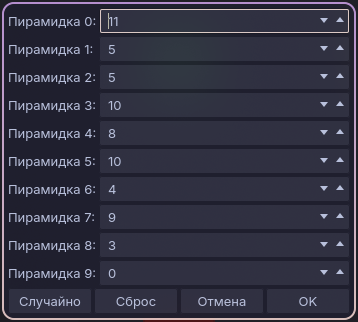
\includegraphics[width=0.5\textwidth]{pics/initial_fill_dialog.png}
  \caption*{Рисунок 3 - Диалог настройки начального количества колец}
\end{figure}

Диалог выбора цветов открывается через меню «Настройки → Выбор цвета». Содержит:

\begin{itemize}
  \item[$-$] \textbf{10 выпадающих списков} (QComboBox) для каждой пирамиды с 14 цветами палитры.
  \item[$-$] \textbf{Цветные иконки} рядом с названиями цветов для визуального выбора.
  \item[$-$] \textbf{Кнопка «Случайно»}: присваивает каждой пирамиде уникальный случайный цвет.
  \item[$-$] \textbf{Кнопка «OK»}: применяет настройки цветов.
  \item[$-$] \textbf{Кнопка «Отмена»}: закрывает диалог без изменений.
\end{itemize}

Логика работы: при выборе цвета в одном списке система проверяет, не используется ли этот цвет другой пирамидой. Если конфликт обнаружен, выводится предупреждение и автоматически выбирается доступный цвет. Кнопка «Случайно» гарантирует уникальность цветов путем случайного перераспределения.

\begin{figure}[H]
  \centering
  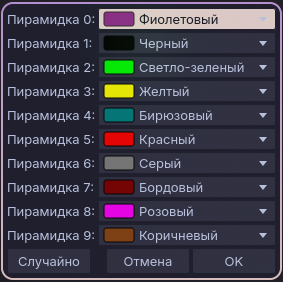
\includegraphics[width=0.5\textwidth]{pics/color_dialog.png}
  \caption*{Рисунок 4 - Диалог выбора цветов пирамид}
\end{figure}

\clearpage

Во время работы симуляции пирамиды анимируются: кольца появляются постепенно, при авариях происходит визуальный эффект тревоги. Статусная строка показывает текущее распределение пирамид по состояниям.

\begin{figure}[H]
  \centering
  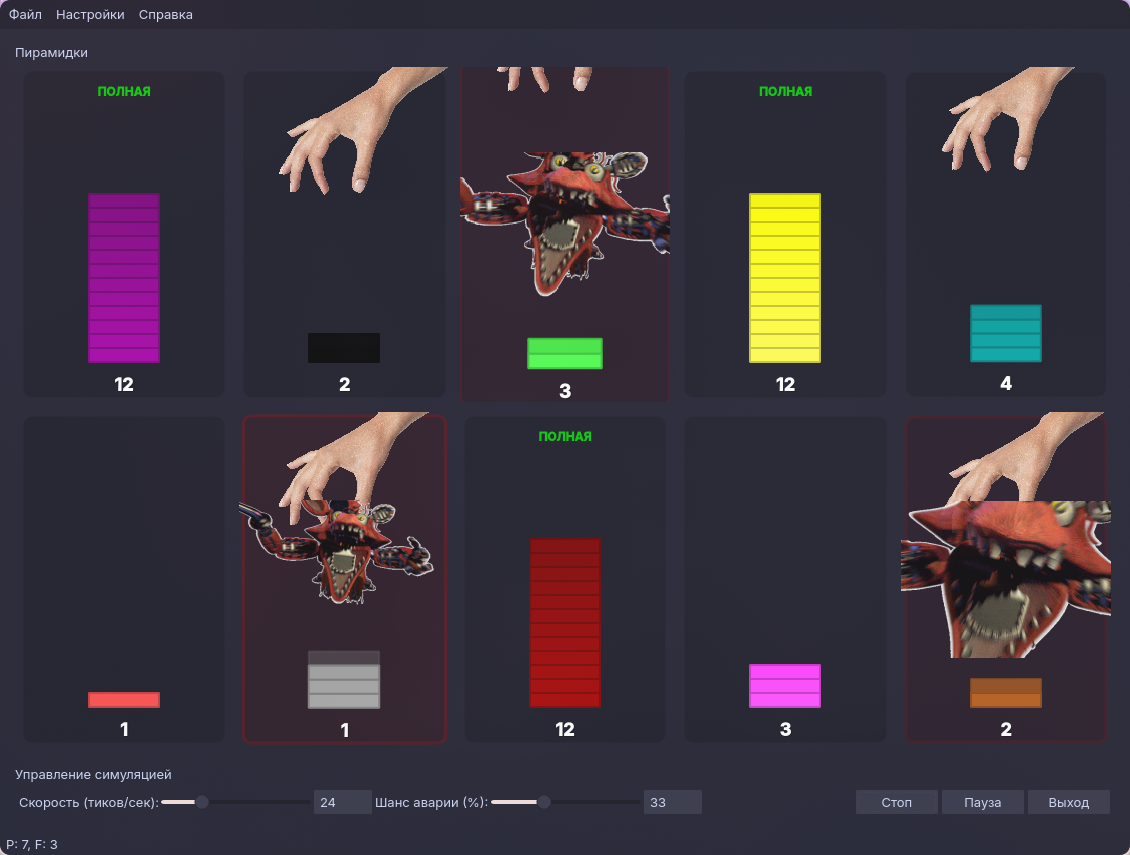
\includegraphics[width=0.95\textwidth]{pics/simulation_running.png}
  \caption*{Рисунок 5 - Процесс симуляции с анимацией}
\end{figure}

\section*{Вывод}

В ходе выполнения лабораторной работы №1 был разработан конечный автомат, моделирующий процесс управления пирамидами с кольцами. Автомат реализует три состояния (O, P, F) и генерирует случайную последовательность входных сигналов в виде добавления колец и аварийных ситуаций.

Приложение создано на фреймворке Qt6 с использованием языка C++. Реализована визуализация состояния автомата с анимацией, диалоги настройки параметров, сохранение и загрузка конфигураций. Код организован в модули с четким разделением ответственности между классами Simulation, MainWindow, PyramidWidget и диалогами.
\end{document}
